\documentclass[a4paper, fontsize=14pt]{article}
\usepackage[T2A]{fontenc}
\usepackage{mathtools}
\usepackage[utf8]{inputenc}
\usepackage[english, russian]{babel}
\usepackage{fancyhdr}
\usepackage{graphicx}
\usepackage{gensymb}
\usepackage{floatrow}
\usepackage{titlesec}
\usepackage{lastpage}
\usepackage{float}
\usepackage{gensymb}
\usepackage{booktabs}
\usepackage{amsmath}
\usepackage{amssymb}

\pagestyle{fancy}
	\fancyhf{}
	\lhead{\hspace{1bp} Работа \textnumero 3.3.1}
	\rhead{Терехов Максим 876\hspace{1bp}}
	\cfoot{\textbf{}}
	\rfoot{\thepage\ \textnormal{из}\ \pageref{LastPage}}
	\renewcommand{\headrulewidth}{1pt}
	\renewcommand{\footrulewidth}{1pt}


%\addtolength{\hoffset}{-1.75cm}
%\addtolength{\textwidth}{3.5cm} 

%\addtolength{\voffset}{-1.5cm}
%\addtolength{\textheight}{3cm} 

\titleformat{\section}
    [block]{\normalfont\bfseries\large}{\rlap{\thesection}}{0em}
    {\vspace{-0.02\textwidth}\begin{minipage}[t]{.95\textwidth}}
[\end{minipage}]

\thispagestyle{fancy}

\begin{document}
\selectlanguage{russian}
\parindent=1cm


\huge
\centering
\textbf{Эффект Холла в металлах}
\raggedright
\large
\section*{Цель работы:}
Измерение подвижности и концентрации носителей заряда в металлах.
\section*{Оборудование:}
Электромагнит с источником питания, источник постоянного тока, микровольтметр Ф116/1б амперметры, милливеберметр, образцы из меди, серебра и цинка.
\section*{Экспериментальная установка:}
\begin{figure}[H]
\center
\includegraphics[scale=0.3]{ust.png}
\caption{Схема установки}
\end{figure}
\section*{Теоретическая часть:}
	Одновременное исследование эффекта Холла и проводимости позволяет находить плотность носителей заряда и их подвижность. Суть эффекта Холла состоит в следующем. Пусть через однородную пластину металла вдоль оси $x$ течет ток $I$. Если эту пластину поместить в магнитное поле, направленно по оси $y$, то между гранями появится раность потенциалов. На электрон, движущийся со скоростью $\mathbf{b}$ в электромагнитном поле, действует сила Лоренца.
		\begin{equation}
			\mathbf{F_\text{л}} = -e\mathbf{E} - e\mathbf{v} \times \mathbf{B}
		\end{equation}
		В нашем случае сила, обусловленная вторым слагаемым, направлена вдоль оси $z$.
		\begin{equation}
			F_B = e\left|v_x\right|B
		\end{equation}
		Под действием этой силы электроны отклоняются к грани Б, заряжая ее отрицательно. При этом на грани А накапливаются нескомпенсированные положительные заряды, что приводит к возникновению электрического поля $E_z$, направленного от А к Б, которое действует на электроныс силой $F_E = eE_z$, направленной против силы $F_B$.  В стационарном режиме $F_E$ уравновешивает $F_B$, и накопление зарядов на боковых гранях прекращается. Из условия равновесия найдем:
		\begin{equation}
			E_z = \left|v_x\right|B
		\end{equation}
		С полем $E_z$ связана разность потенциалов $U_{\text{АБ}}$ между гранями А и Б.
		\begin{equation}
			U_{\text{АБ}} = - E_zl = - \left|v_x\right|Bl
		\end{equation}
		Заметим, что сила тока
		\begin{equation}
			I = ne\left|v_x\right|l\cdot a,
		\end{equation}
		отсюда найдем ЭДС Холла:
		\begin{equation}
			U_x = U_{\text{АБ}} = -\frac{IB}{nea} = -R_x\cdot\frac{IB}{a},
		\end{equation}
		где $R_x = \frac{1}{n e}$ --- постоянная Холла.
\section*{Обработка результатов измерений:}
Построим график зависимости индукции магнитного поля от тока через магнит:
\begin{table}[H]

	\centering
	\begin{tabular}{|c|c|c|c|c|c|c|c|c|c|c|} \hline
		$I_\text{м}, A$ & 0,10 & 0,24 & 0,35 & 0,46 & 0,56 & 0,75 & 0,92 & 1,12 & 1,24 \\\hline
		$b, \text{мТл}$ & 125 & 284 & 408 & 536 & 651 & 751 & 850 & 1050 & 1083 \\\hline
	\end{tabular}	
\end{table}
\begin{figure}[H]
\center
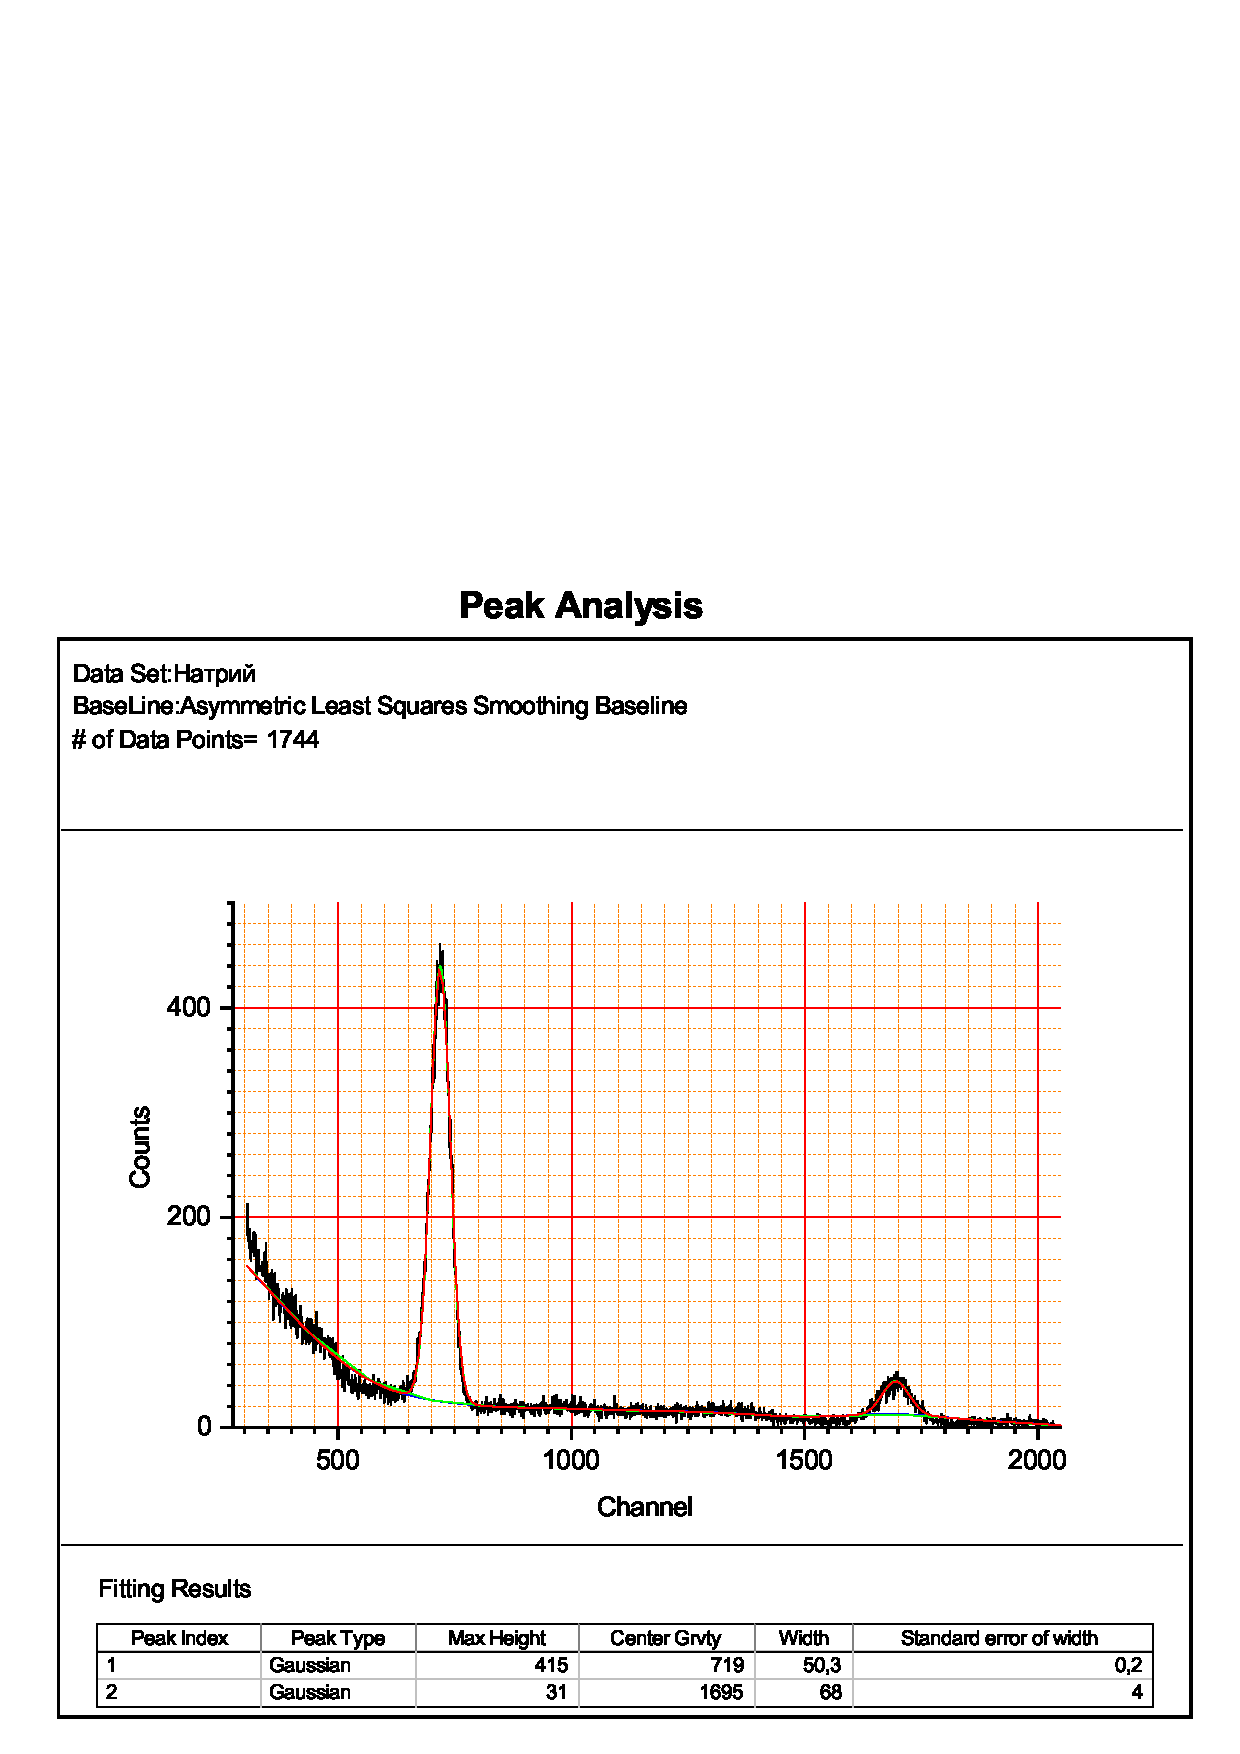
\includegraphics[scale=0.4]{1.png}
\caption{Зависимость $B$ от $I_\text{м}$}
\end{figure}
Построим на одном графике семейство характеристик $U_x = f(B)$ при разных значениях тока $I$ через образец и определим угловые коэффициенты:
\begin{figure}[H]
\center
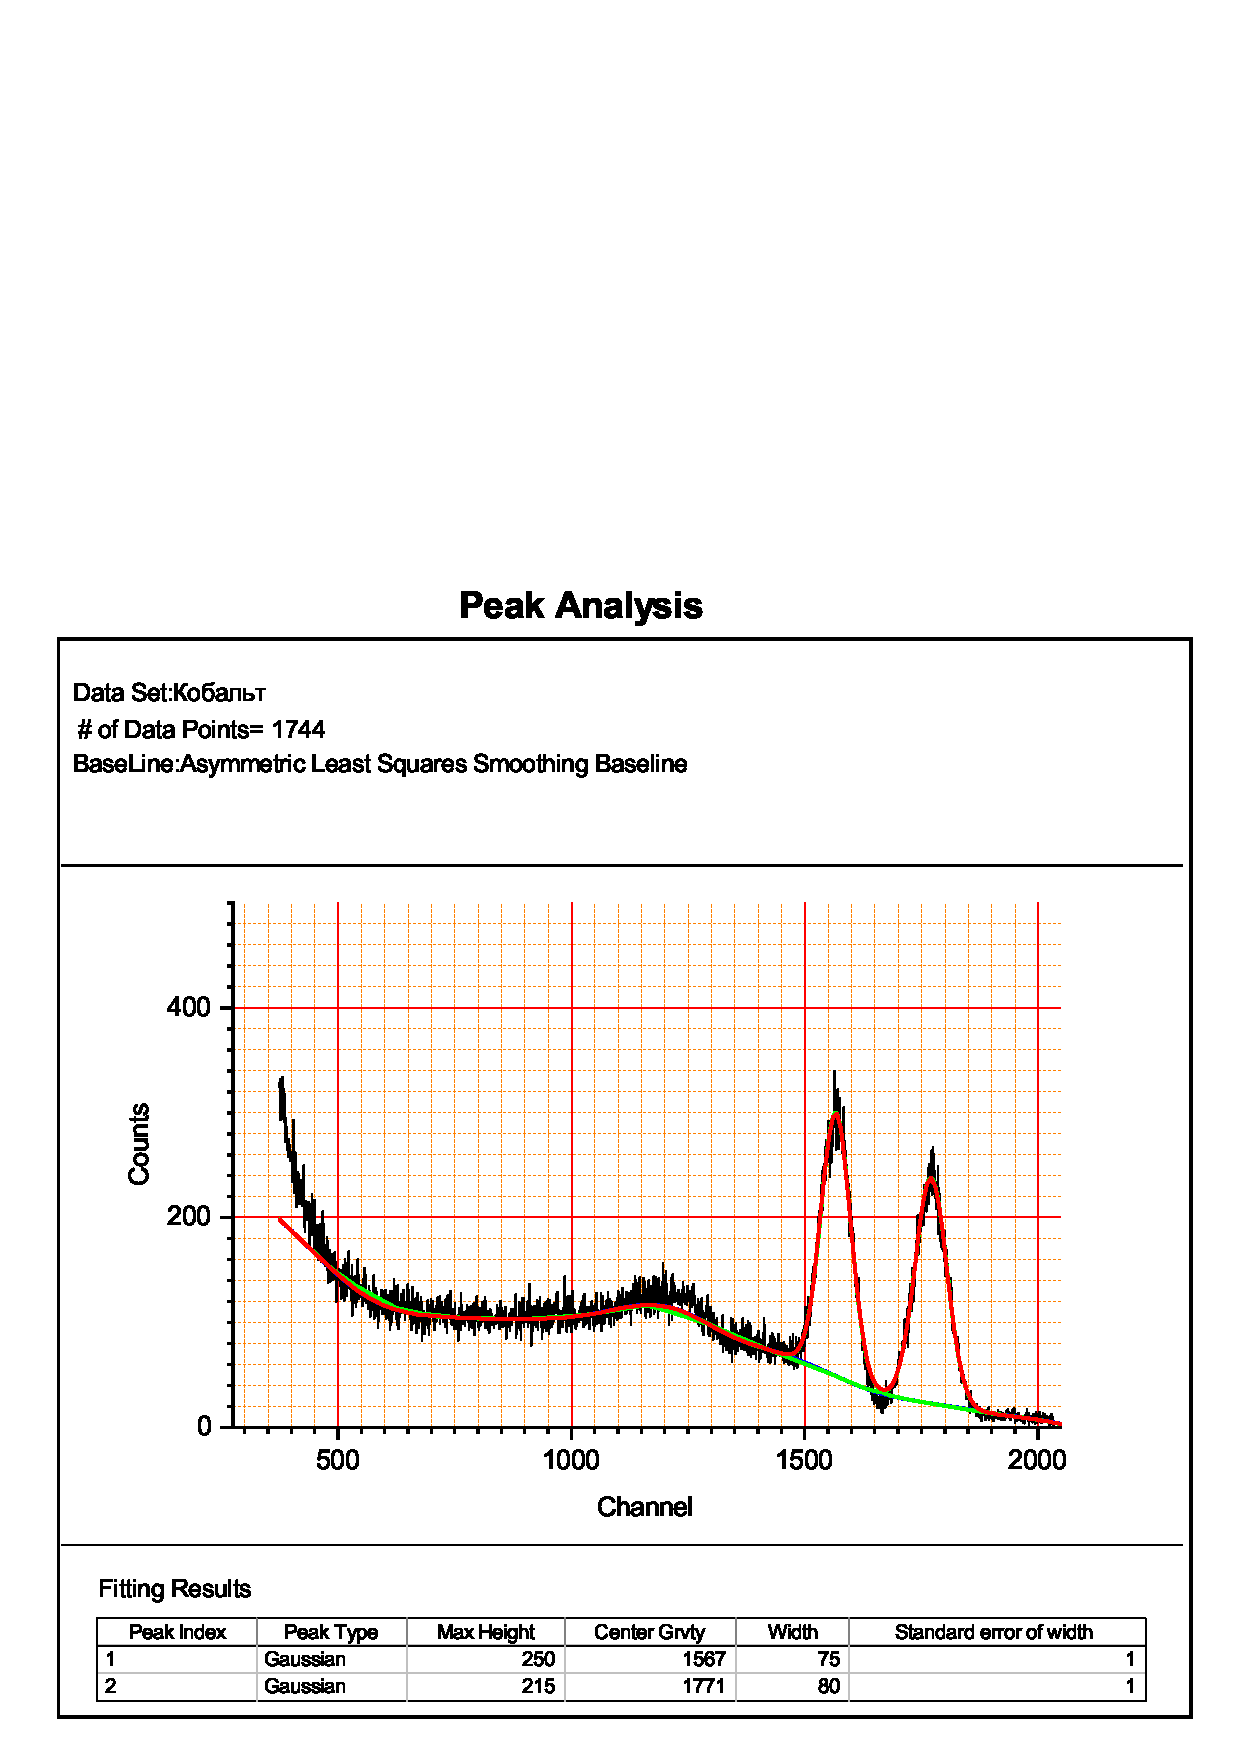
\includegraphics[scale=0.4]{2.png}
\caption{Зависимость $U_x$ от $B$}
\end{figure}
\begin{table}[H]

	\centering
	\begin{tabular}{|c|c|c|c|c|c|} \hline
		$K, 10^{-4}\ \frac{\Delta U_x}{\Delta B}$ & 6.1 & 7.0 & 8.3 & 9.4 & 12.8 \\\hline
	\end{tabular}	
\end{table}
Построим график зависимости коэффициента наклона от тока через образец и из него определим величину постоянной Холла $R_x$:
\begin{figure}[H]
\center
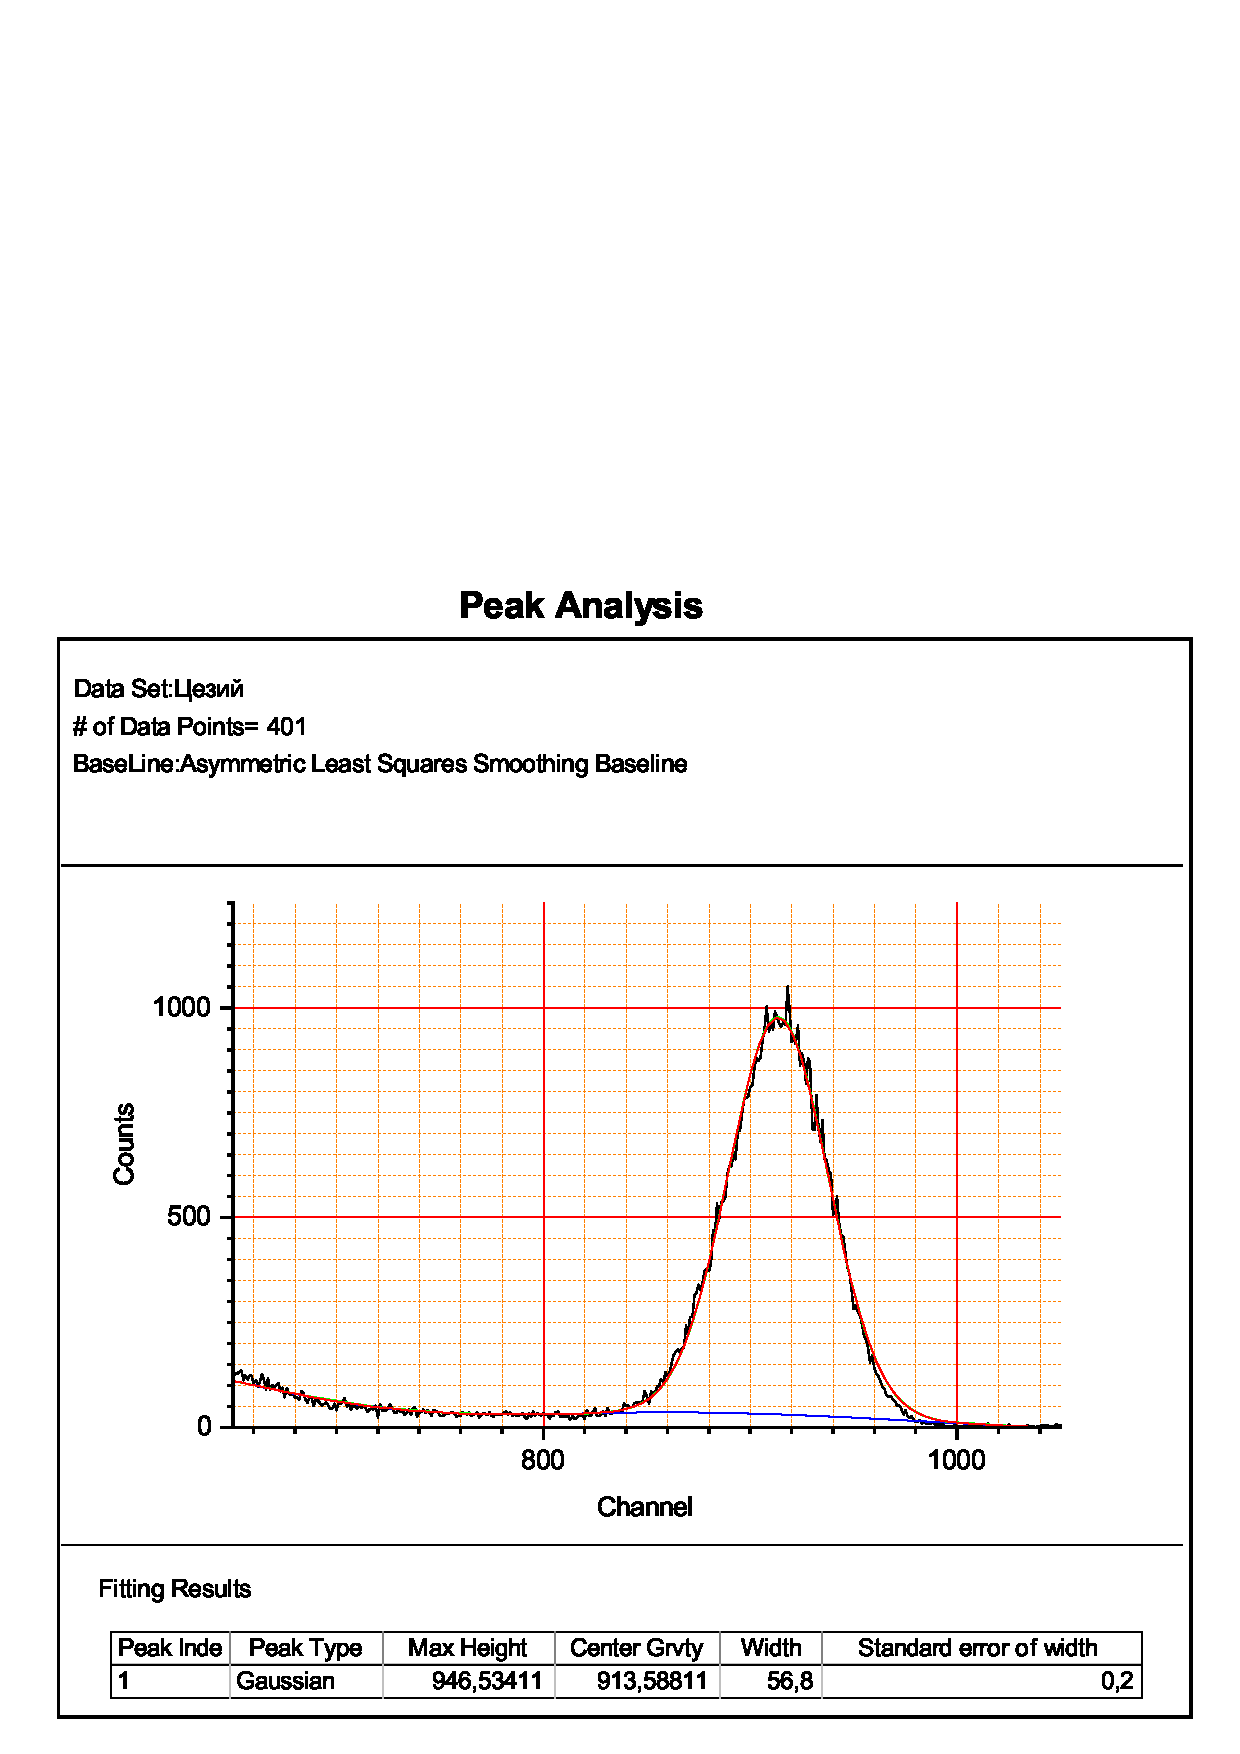
\includegraphics[scale=0.4]{3.png}
\caption{Зависимость $k$ от $I$}
\end{figure}
Коэффициент наклона графика $K = 11.8 \pm 0.3$
\[
	R_x = - \frac{K}{a} = -0.87 \pm 0.3\ \frac{\text{м}^3}{\text{Кл}}
\]
Табличное значение $R_{x_\text{табл}} = -0.9\ \frac{\text{м}^3}{\text{Кл}}$
\section*{Вывод:}
Найденная нами постоянная Холла с учётом погрешности совпадает с табличной. Знак этой постоянной показывает, что основными носителями заряда в металле являются электроны.
\end{document}